\documentclass{beamer}
\usepackage{ulem}
\usepackage{tikz}
\usepackage{booktabs}
 \usepackage{graphicx,threeparttable,caption}
\usetikzlibrary{shapes,snakes}
\usepackage[beamer,customcolors]{hf-tikz}
\usepackage{nicematrix}
\usepackage{xcolor}
\usepackage{makecell}
\usepackage{array}
\usepackage{csquotes}
\usepackage{csquotes}
\usepackage{minted}
\captionsetup{labelformat=empty,labelsep=none}

\graphicspath{ {./png/} }
\tikzset{hl/.style={
    set fill color=red!80!black!40,
    set border color=red!80!black,
  },
}
\AtBeginSection[]{
  \begin{frame}
  \vfill
  \centering
  \begin{beamercolorbox}[sep=8pt,center,shadow=true,rounded=true]{title}
    \usebeamerfont{title}\insertsectionhead\par%
  \end{beamercolorbox}
  \vfill
  \end{frame}
}
\definecolor{pinkWybory}{RGB}{224, 101, 137}
%\usecolortheme[named = pinkWybory]{structure}
\usetheme[hideothersubsections]{PaloAlto}
\makeatletter
\patchcmd{\csq@bquote@i}{{#6}}{{\emph{#6}}}{}{}
\makeatother
%\usecolortheme{orchid}
%\usefonttheme{professionalfonts}
\newcommand{\soutthick}[1]{%
   \textcolor{red}{
   \renewcommand{\ULthickness}{1pt}%
      \sout{#1}%
   \renewcommand{\ULthickness}{.4pt}% Resetting to ulem default
   }
}
\newcommand{\centered}[1]{\begin{tabular}{l} #1 \end{tabular}}
\setbeamertemplate{section in toc}[square]
\setbeamertemplate{subsection in toc}[square]
\setbeamertemplate{secion in sidebar}[shaded]
\setbeamertemplate{items}[square]
\setbeamercovered{transparent} 

\title[]{Computational Social Science: An Introduction to Data Science}
\subtitle{Introduction}
\author[]{Mikołaj Biesaga\\ \small{\color{blue}{\href{mailto:m.biesaga@uw.edu.pl}{m.biesaga@uw.edu.pl}}}}
\institute{
\includegraphics[width = 4 cm]{uw.png}}
\date{\today}
\begin{document}
\begin{frame}
   \titlepage
\end{frame}

\begin{frame}
    \frametitle{Mikołaj Biesaga}
    \only<1>{
        \framesubtitle{Best Book Ever}
        \begin{center}
            
\includegraphics[width = .4\textwidth]{gww.jpg}
        \end{center}
    }
    \only<2>{
        \framesubtitle{Current book}
        \begin{center}
            
\includegraphics[width = .5\textwidth]{7killings.jpg}
        \end{center}
    }
    \only<3>{
        \framesubtitle{Current comics book}
        \begin{center}
            
\includegraphics[width = .5\textwidth]{alvar.jpg}
        \end{center}
    }

    %% \only<4>{
    %%     \framesubtitle{Frequency in General Elections}
    %%     \begin{center}
    %%         \includegraphics[width = .5\textwidth]{wybory.png}
    %%     \end{center}
    %% }
\end{frame}

\section{Rules of Engagement}

\begin{frame}
    \frametitle{Office Hours, Emails, Presentations, etc.}
    \begin{description}[Google Classroom:]
        \item [Office Hours:] write me an email before coming
        \item [Emails:] the official info will go through emails
        \item [GitHub:] scripts (notebooks) will be posted on GitHub
        \item [Google Classroom:] materials and presentations will be posted on
        Google Drive
    \end{description}
    \alert{I will try to answer your inquiries as soon as possible but do not
    count on an immediate response, especially right before the deadlines.}
\end{frame}
\begin{frame}
    \frametitle{Emails}
    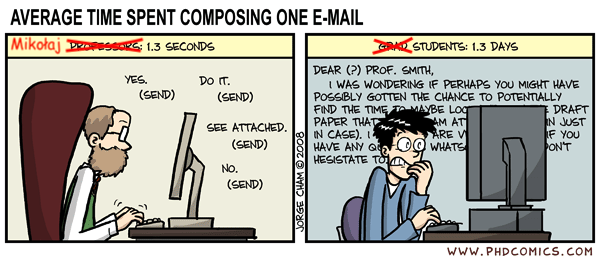
\includegraphics[width = \textwidth]{emails.png}
\end{frame}
\begin{frame}
    \frametitle{Workflow}
    \begin{enumerate}
        \item Presentation of the basic concepts in the classroom.
        \item Exercises in the classroom.
        \item Homework assignments requiring modifying the work done in the
        classroom.
        \item Final research project.
    \end{enumerate}
\end{frame}
\begin{frame}
    \frametitle{Assessment Criteria}
    \begin{itemize}
        \item The final grade will be determined based on \alert{3 homework
        assignments} and a \alert{written research project proposal}.
        \item All 3 homework (after classes: 6, 9, and 13) will be scored from 0
        to 15 points.
        \item The research project will require writing a research proposal that
        uses tools and methods we will use during the course. It will be scored
        from 0 to 55 points.
        \item Grading criteria:
    \begin{description}
        \item [5\phantom{+} --] => 90 points
        \item [4+ --] 85 - 89 points
        \item [4\phantom{+} --] 75 - 84 points
        \item [3+ --] 70 - 74 points
        \item [3\phantom{+} --] 60 - 69 points
        \item [2\phantom{+} --] =< 59 points
    \end{description}
\end{itemize}
\end{frame}
\begin{frame}
    \frametitle{Attendance}
    \only<1>{
        \begin{itemize}
            \item Attendance is advised.
            \item You are allowed to miss up to \alert{2 classes without a formal excuse}.
            \item Additionally, you are allowed to miss up to \alert{2 classes in case of a formal
            excuse}.
            \item An absence does not exempt from doing homework assignments.
        \end{itemize}
    }
    \only<2>{
        \begin{center}
            
\includegraphics[width = .9\textwidth]{png/pretty_please.jpg}
        \end{center}
    }
\end{frame}

\begin{frame}
    \frametitle{Additional Resources}
    \only<1>{
        \begin{center}
            
\includegraphics[width = .5\textwidth]{copy_paste.png}
        \end{center}
    }
    \only<2>{
        \begin{center}
            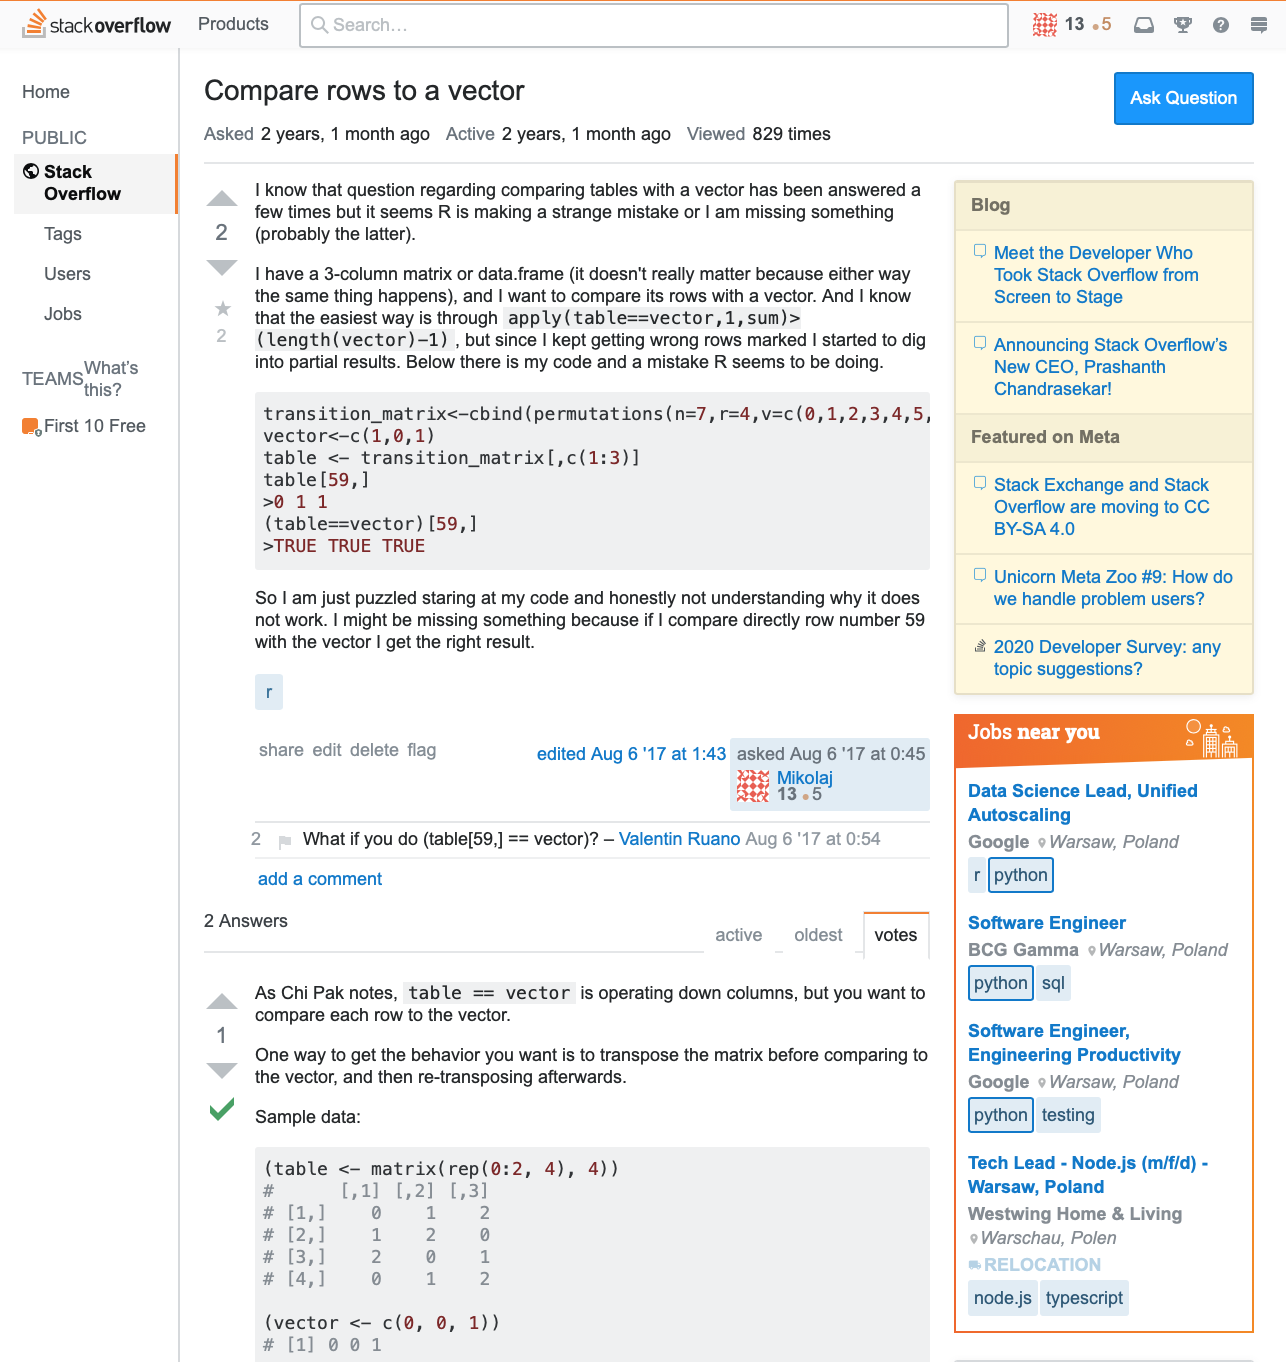
\includegraphics[width = .6\textwidth]{stack_overflow.png}
        \end{center}
    }
    \only<3>{
        \begin{itemize}
            \item \textcolor{blue}{\href{https://stackoverflow.com}{www.stackoverflow.com}}
            \item \textcolor{blue}{\href{https://www.learnpython.org}{www.learnpython.org}}
        \end{itemize}
    }
    \only<4>{
        \begin{center}
            
\includegraphics[width = .9\textwidth]{chatgpt_meme_original.jpg}
        \end{center}
    }
    \only<5>{
        \begin{center}
            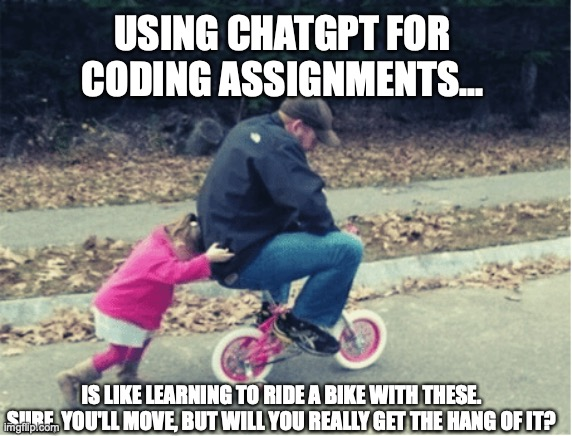
\includegraphics[width = .8\textwidth]{chatgpt_meme2.jpg}
        \end{center}
    }
    \only<6>{
        \begin{center}
            
\includegraphics[width = .7\textwidth]{dalle-meme.png}
        \end{center}
    }
    
\end{frame}

\section[CSS]{Computational Social Science}

\begin{frame}
    \frametitle{What is Computational Social Science?}
    \begin{definition}{}
        In the most general sense \emph{Computational Social Science} is a data-driven approach that uses computational methods in studying social phenomena.
    \end{definition}
    \begin{definition}{}
        \emph{Data Science} on the other hand is a broader term than Computational Social Science. It describes the theory and practice of extracting knowledge and insight from data.
    \end{definition}
\end{frame}

\begin{frame}{General interest in data science}
    \begin{figure}
    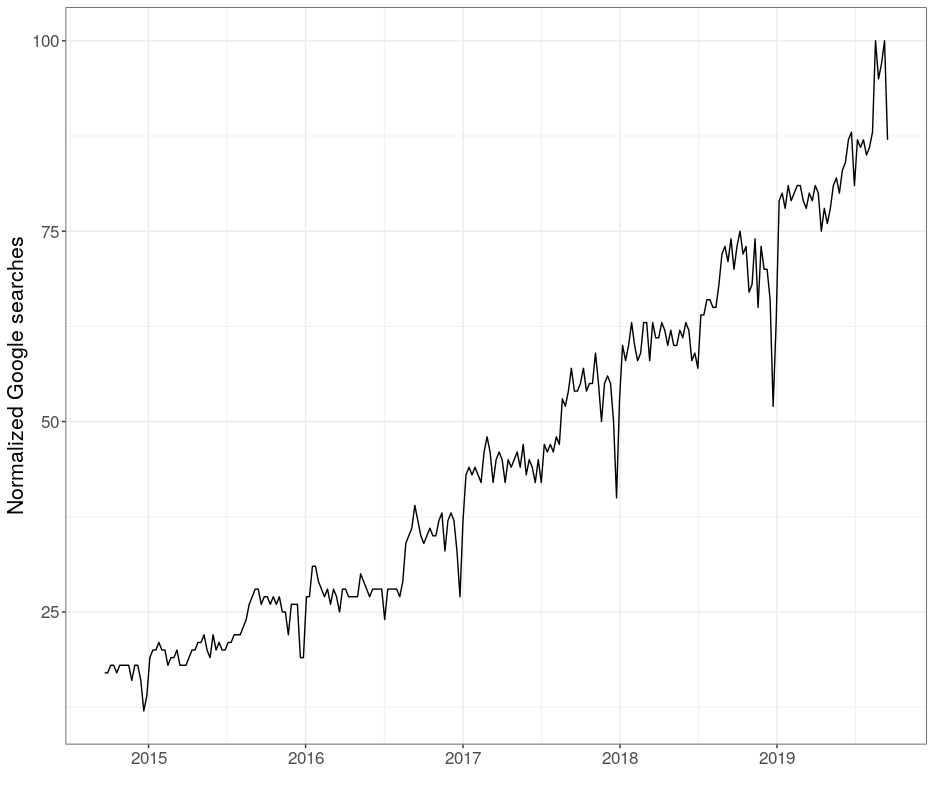
\includegraphics[width = .8\framewidth]{png/ds-searches.png}
    \caption{Growth of "data science" Google search}
    \end{figure}
\end{frame}

\subsection{Research Methods}

\begin{frame}
    \frametitle{Traditional Research Methods}
        \only<0>{
            \begin{figure}
                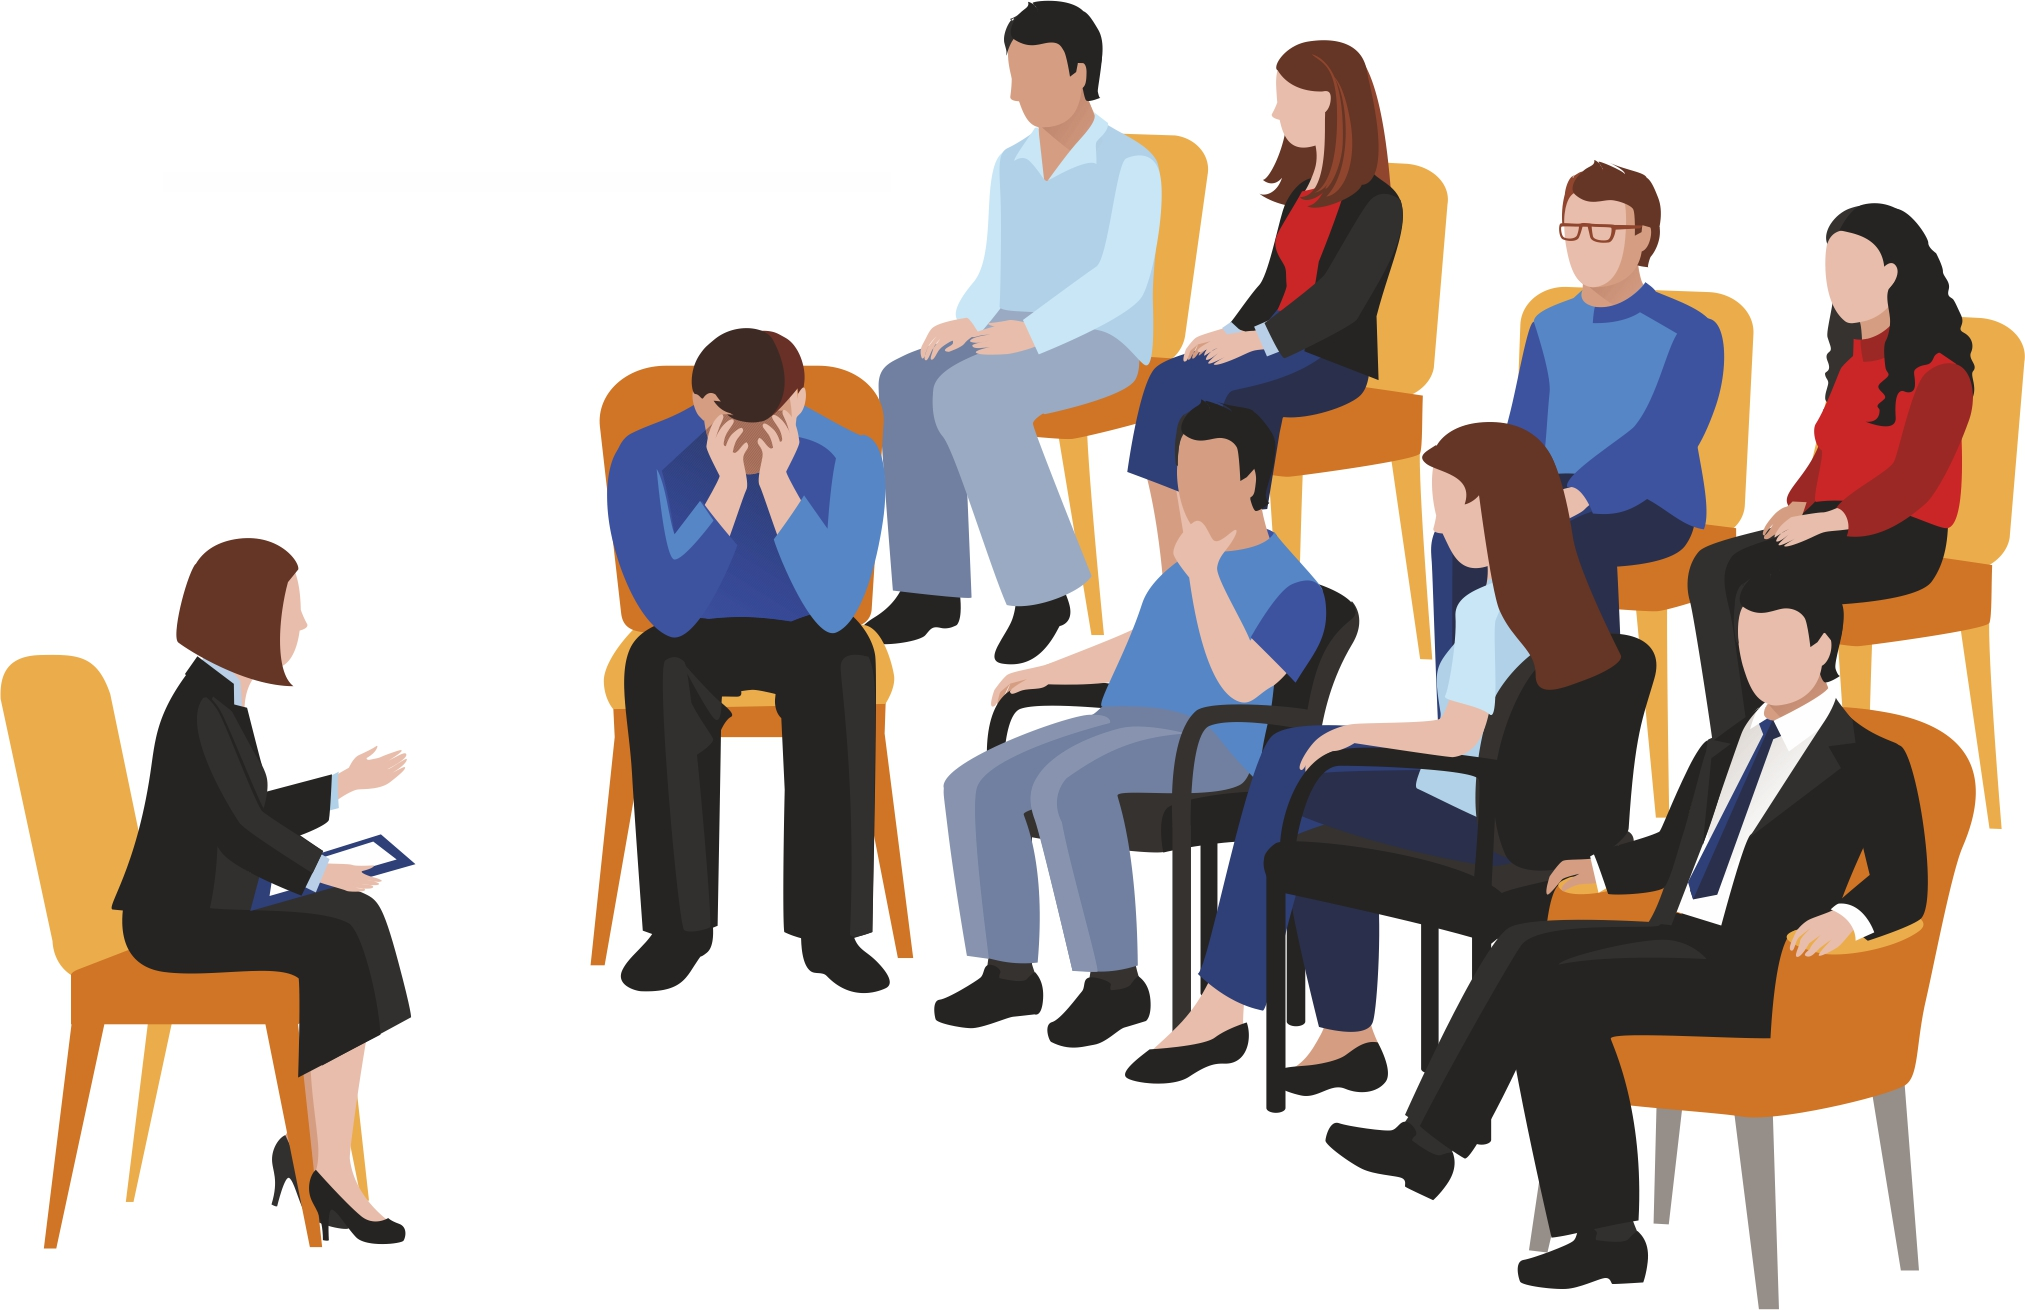
\includegraphics[scale = .5]{png/traditional.jpg}
            \end{figure}
        }
        \only<+>{
            \begin{itemize}
                \item surveys
                \item observational studies
                \item experiments
                \item case studies
                \item event sampling methodology (diaries)
                \item interviews
                \item meta-analysis
            \end{itemize}}
        \only<+>{
            \resizebox{\textwidth}{!}{
                \begin{tabular}{l | c | c | c | c | c | c }
                Id & Sex & Age & Condition & Variable A & Variable B & Variable C\\
                \hline \hline
                AAA & M & 24 & exp & 55:53 & 3 & apple\\
                AAB & F & 22 & exp & 53:47 & 2 & banana\\
                AAC & F & 28 & con & n/a   & 4 & banana\\
                AAD & M & 21 & con & 54:35 & 3 & banana
                \end{tabular}}
        }
\end{frame}

\begin{frame}
    \frametitle{Computational methods}
    \setbeamercovered{transparent}
    \begin{itemize}
        \item<1> extraction of unstructured data from external digital (i.e. web-based) sources
        \begin{itemize}
            \item<1> webscraping (extraction of data from existing webpages)
            \item<1> extracting data from web APIs (i.e. Twitter)
        \end{itemize}
        \item<1> analysis of textual data (natural language processing - NLP)
        \item<0> network and relational data analysis
        \item<0> working with big datasets (that do not fit into the RAM of a single computer), in-database computations, distributed computing, etc.
        \item<0> computer simulations
        \item<0> online experiments (experiments based on online games etc.)
    \end{itemize}
\end{frame}

\section[Data]{Data}

\subsection[Data Sources]{Data Sources}
\begin{frame}
    \setbeamercovered{transparent}
    \frametitle{Data Sources}
    \only<+>{
        \begin{figure}
            
\includegraphics[scale=.35]{png/data_everywhere.png}
        \end{figure}}
    \only<+>{
        \begin{figure}
            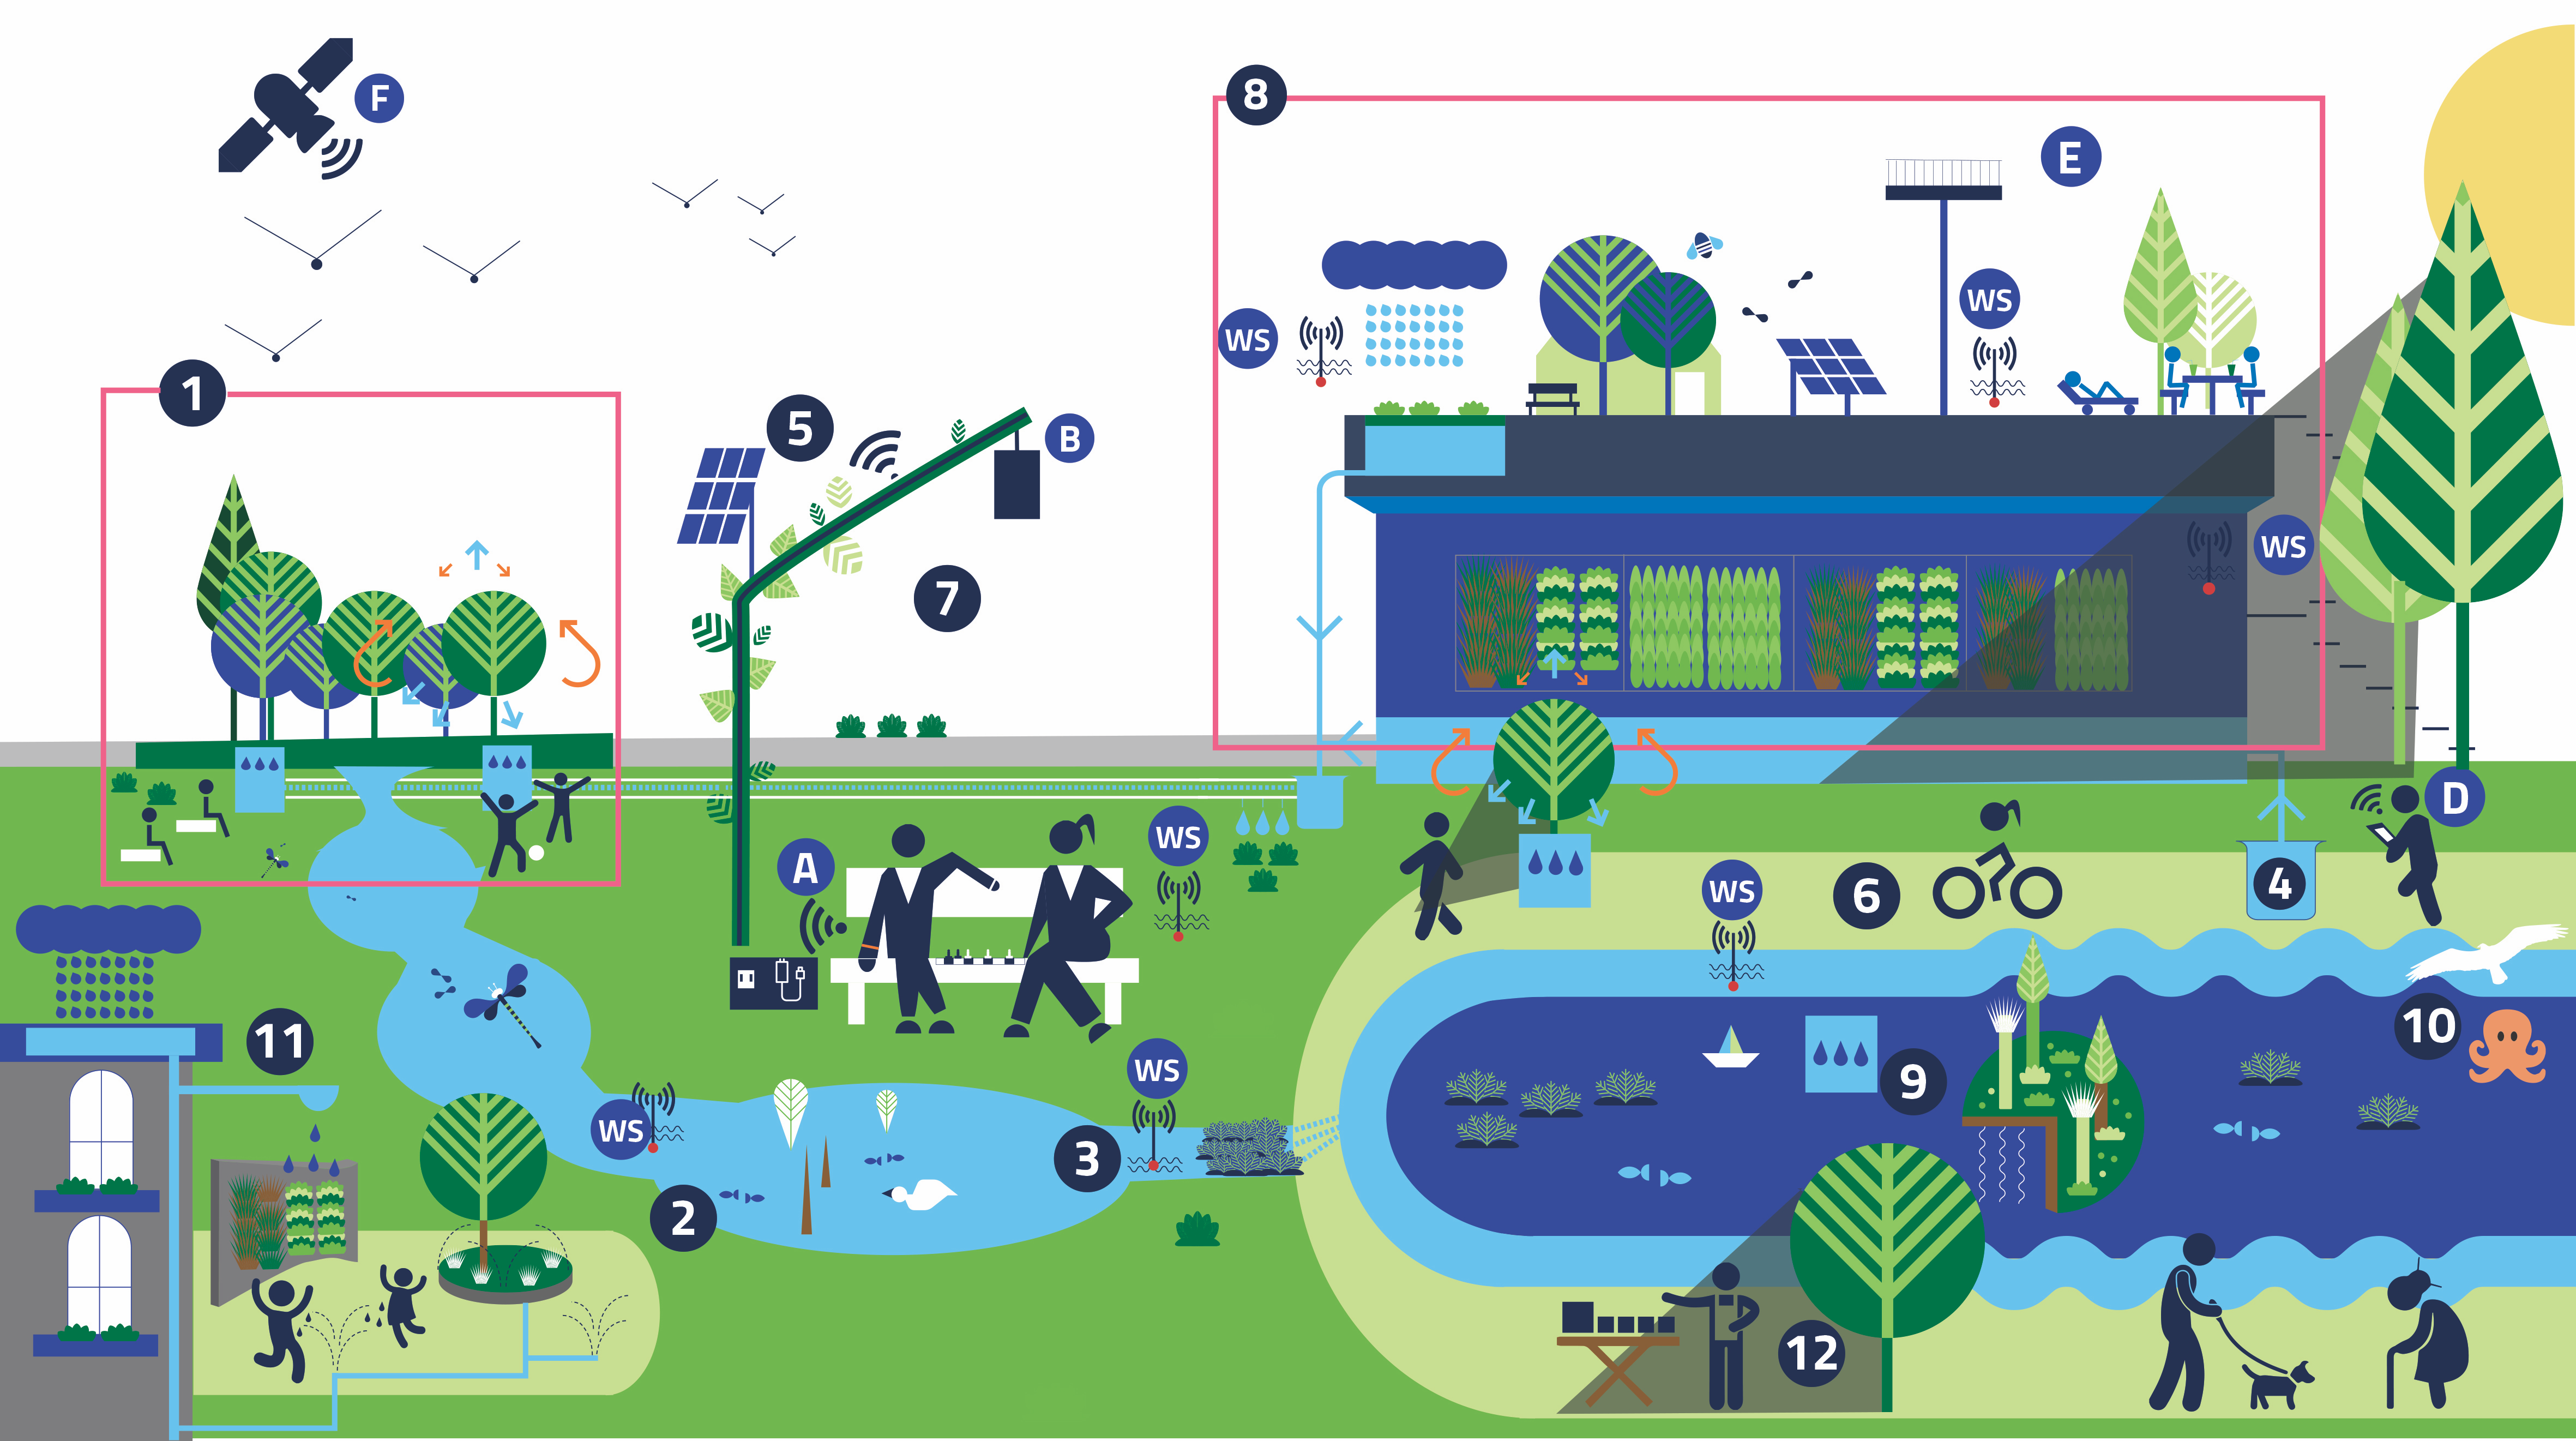
\includegraphics[width = \textwidth]{png/mierzenie.png}
        \end{figure}
    }
    \only<+>{
        \begin{figure}
            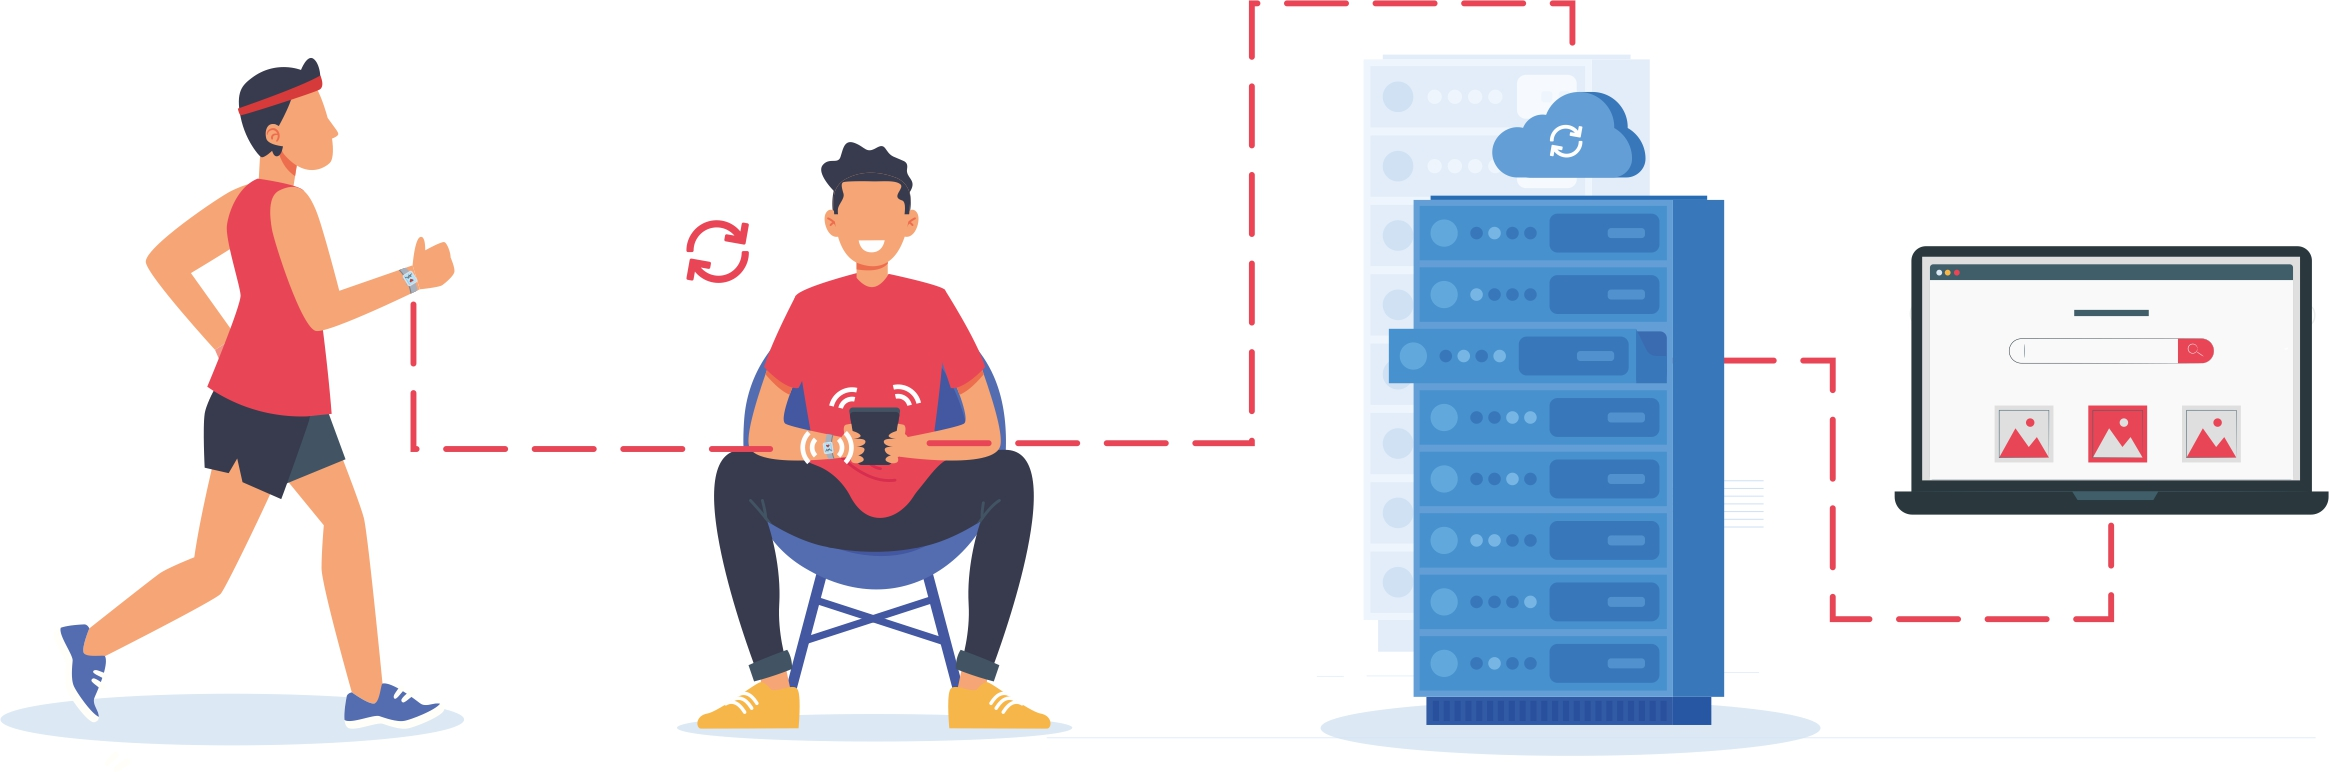
\includegraphics[scale = .5]{png/tracker.jpg}
        \end{figure}
    }
    \only<+>{
        \begin{itemize}
            \item<4> webpages
            \item<4> social media
            \item<0> smart devices
            \item<0> digital behavioral data
            \item<0> mobile phone networks
            \item<0> goverment data
            \item <0>...
        \end{itemize}
        \action<4>{\alert{The fact that you can get the data does not mean you should.}}
    }
\end{frame}

\subsection{Webscraping}

\begin{frame}
    \frametitle{Webscraping}
    \only<+>{
        \begin{figure}
            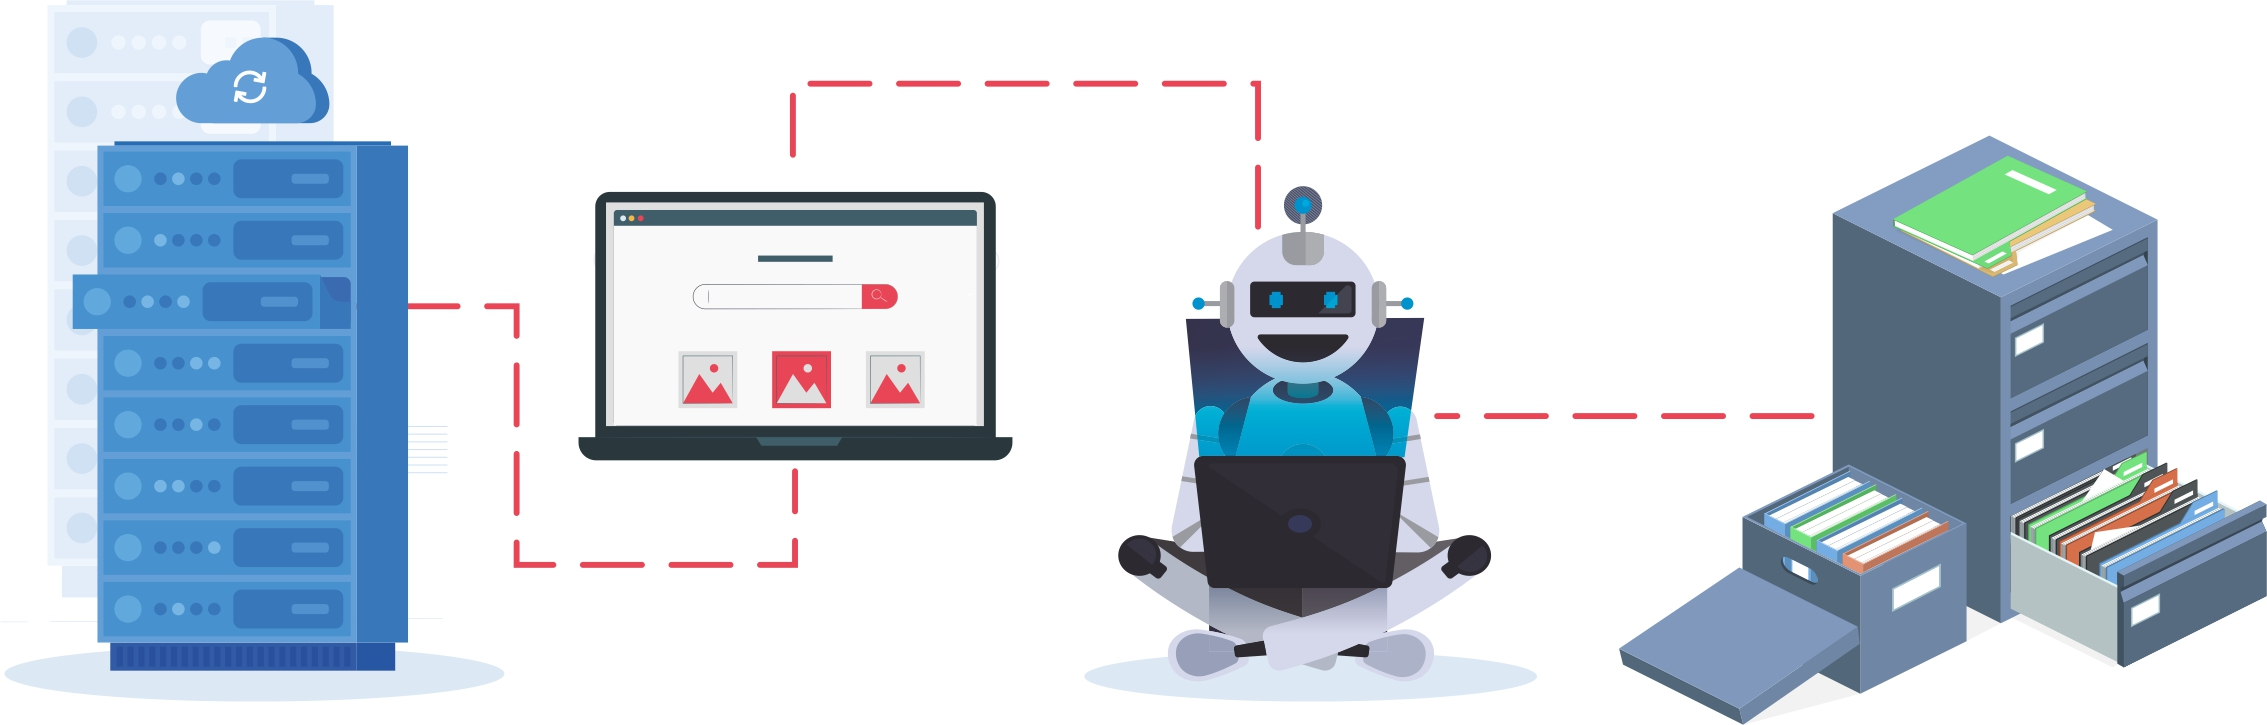
\includegraphics[scale = .5]{png/webscraping.jpg}
        \end{figure}
    }
    \only<+>{
        \begin{figure}
            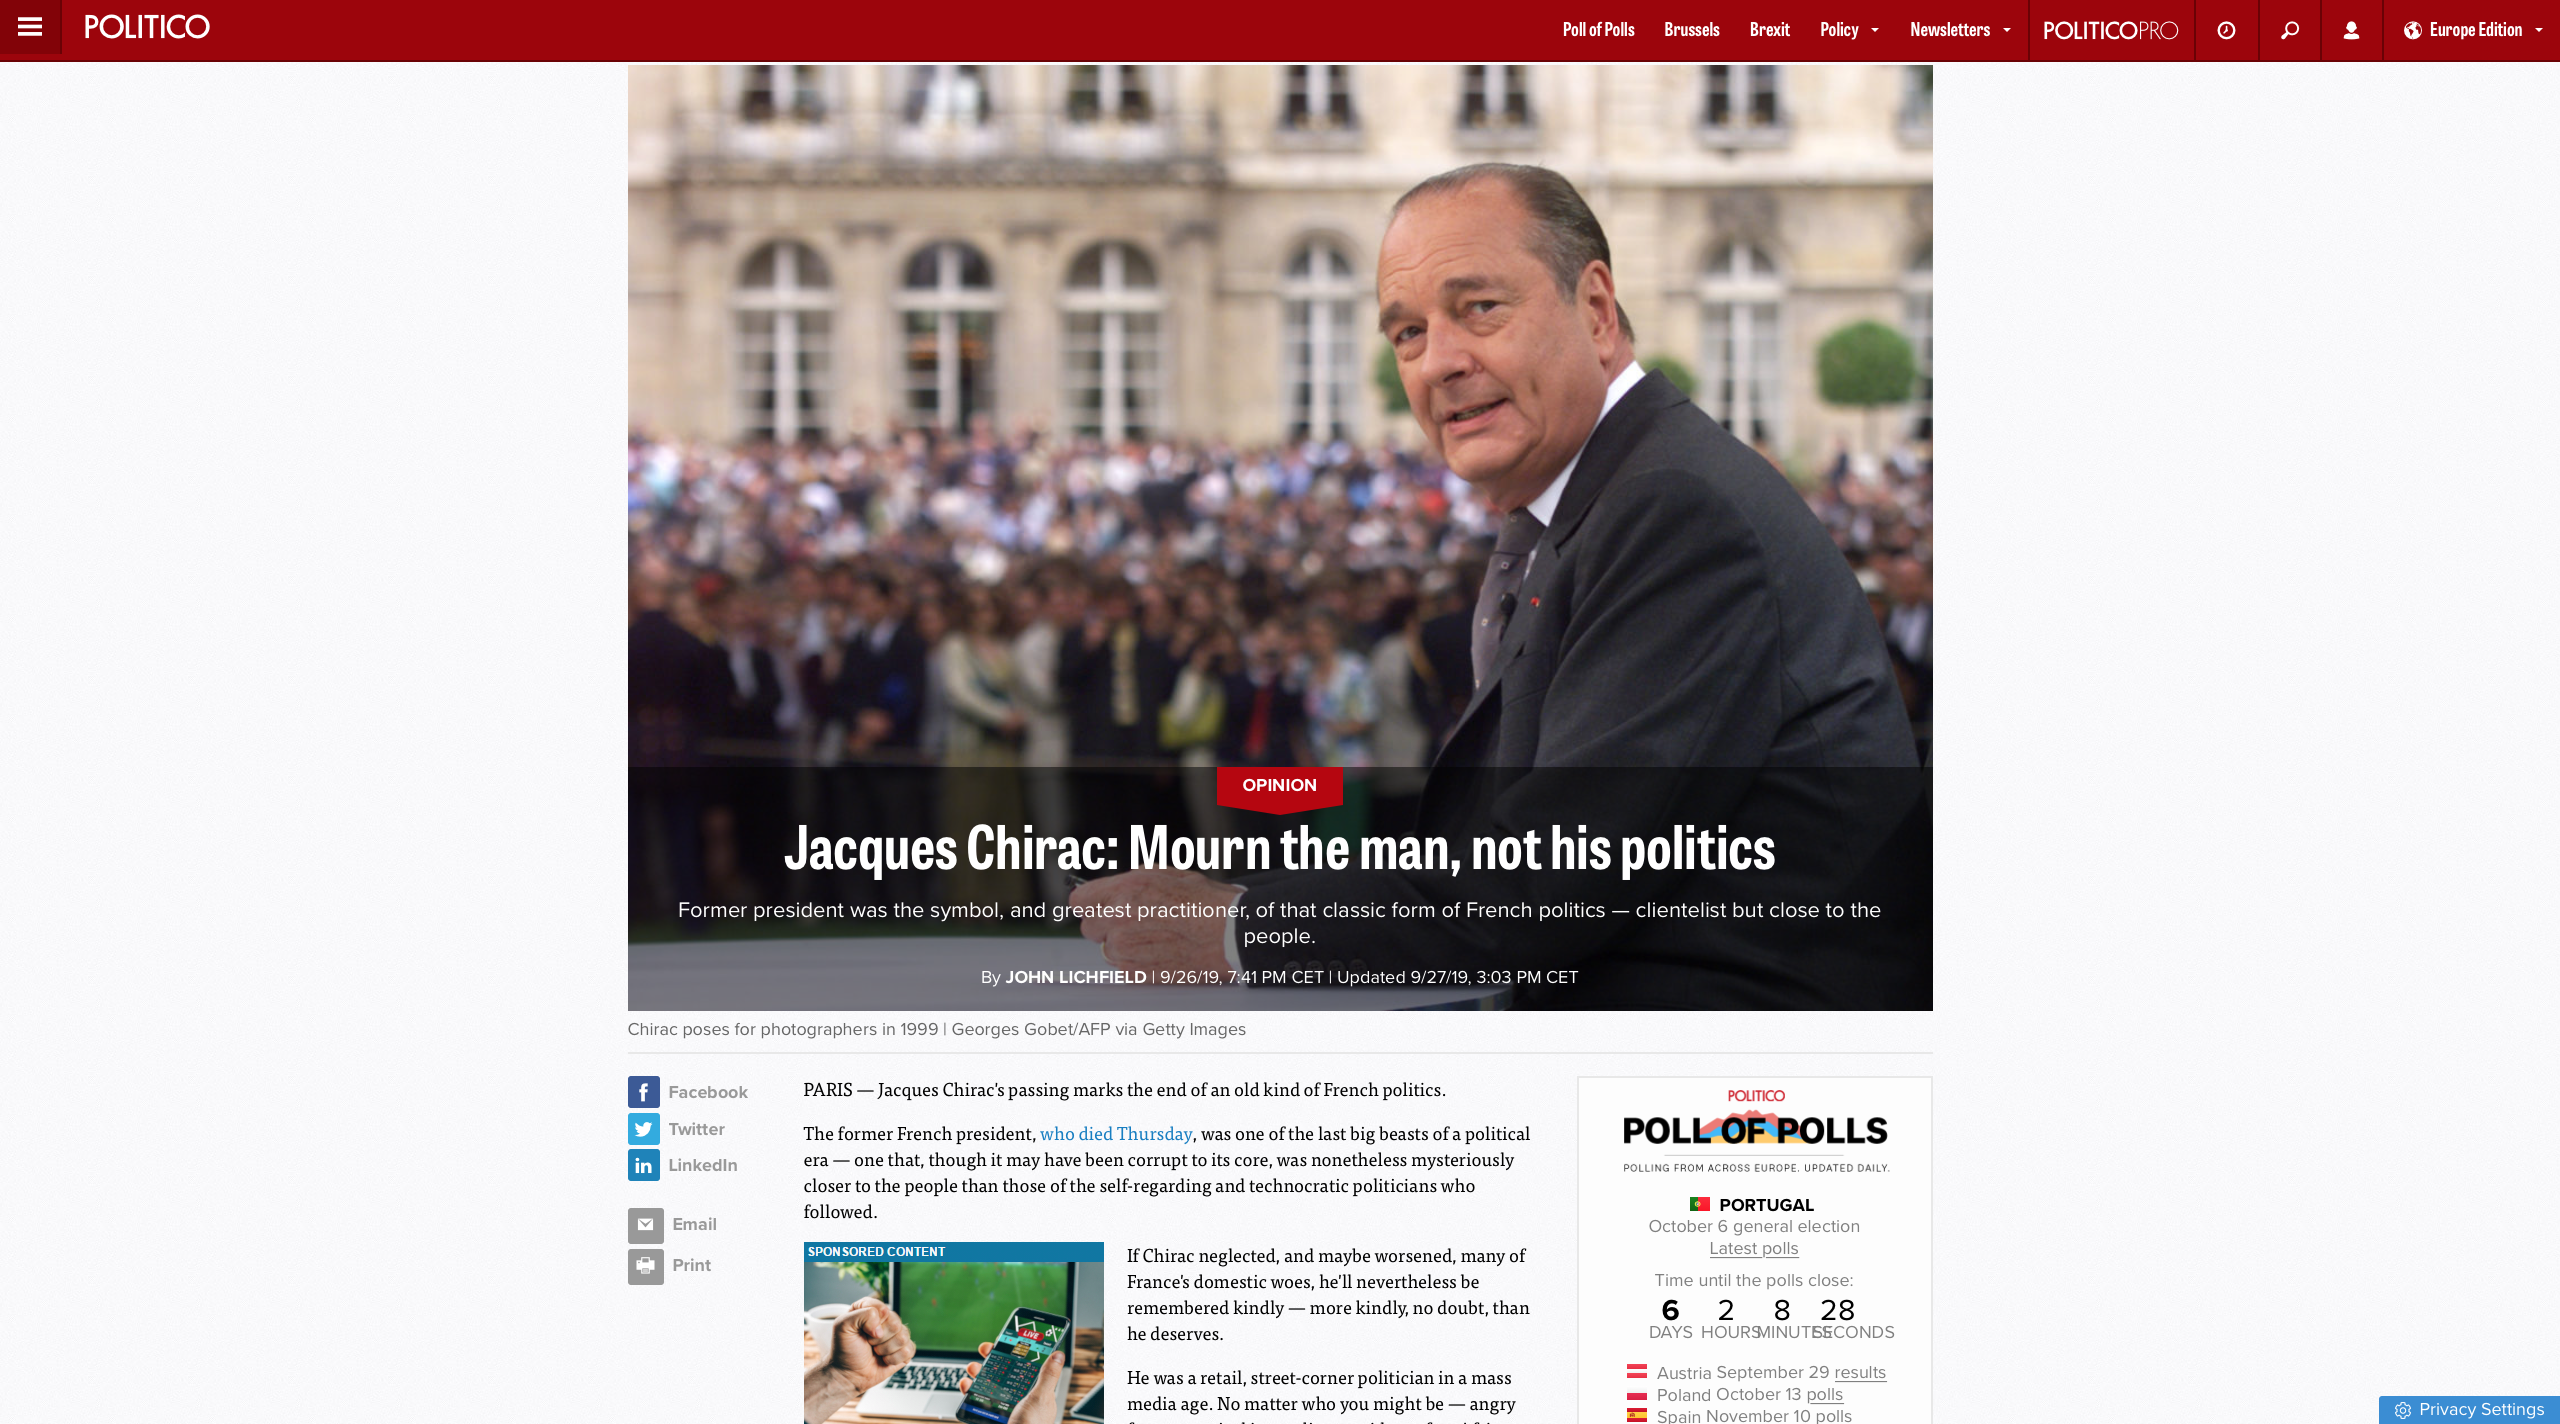
\includegraphics[scale = .22]{png/politico.png}
            \caption{from \textcolor{blue}{\href{https://www.politico.eu/article/jacques-chirac-mourn-the-man-not-his-politics/}{POLITICO Europe}}}
        \end{figure}
    }
    \only<+>{
        \begin{definition}
            \emph{Webscraping} is a process of (usually) automatic extraction of data from a website or multiple websites. In other words, it is a form of copying the data from a website into a local database or spreadsheet.
        \end{definition}
    }
\end{frame}

\subsection{API}

\begin{frame}
    \frametitle{Application Programming Interface}
    \only<+>{
        \begin{figure}
            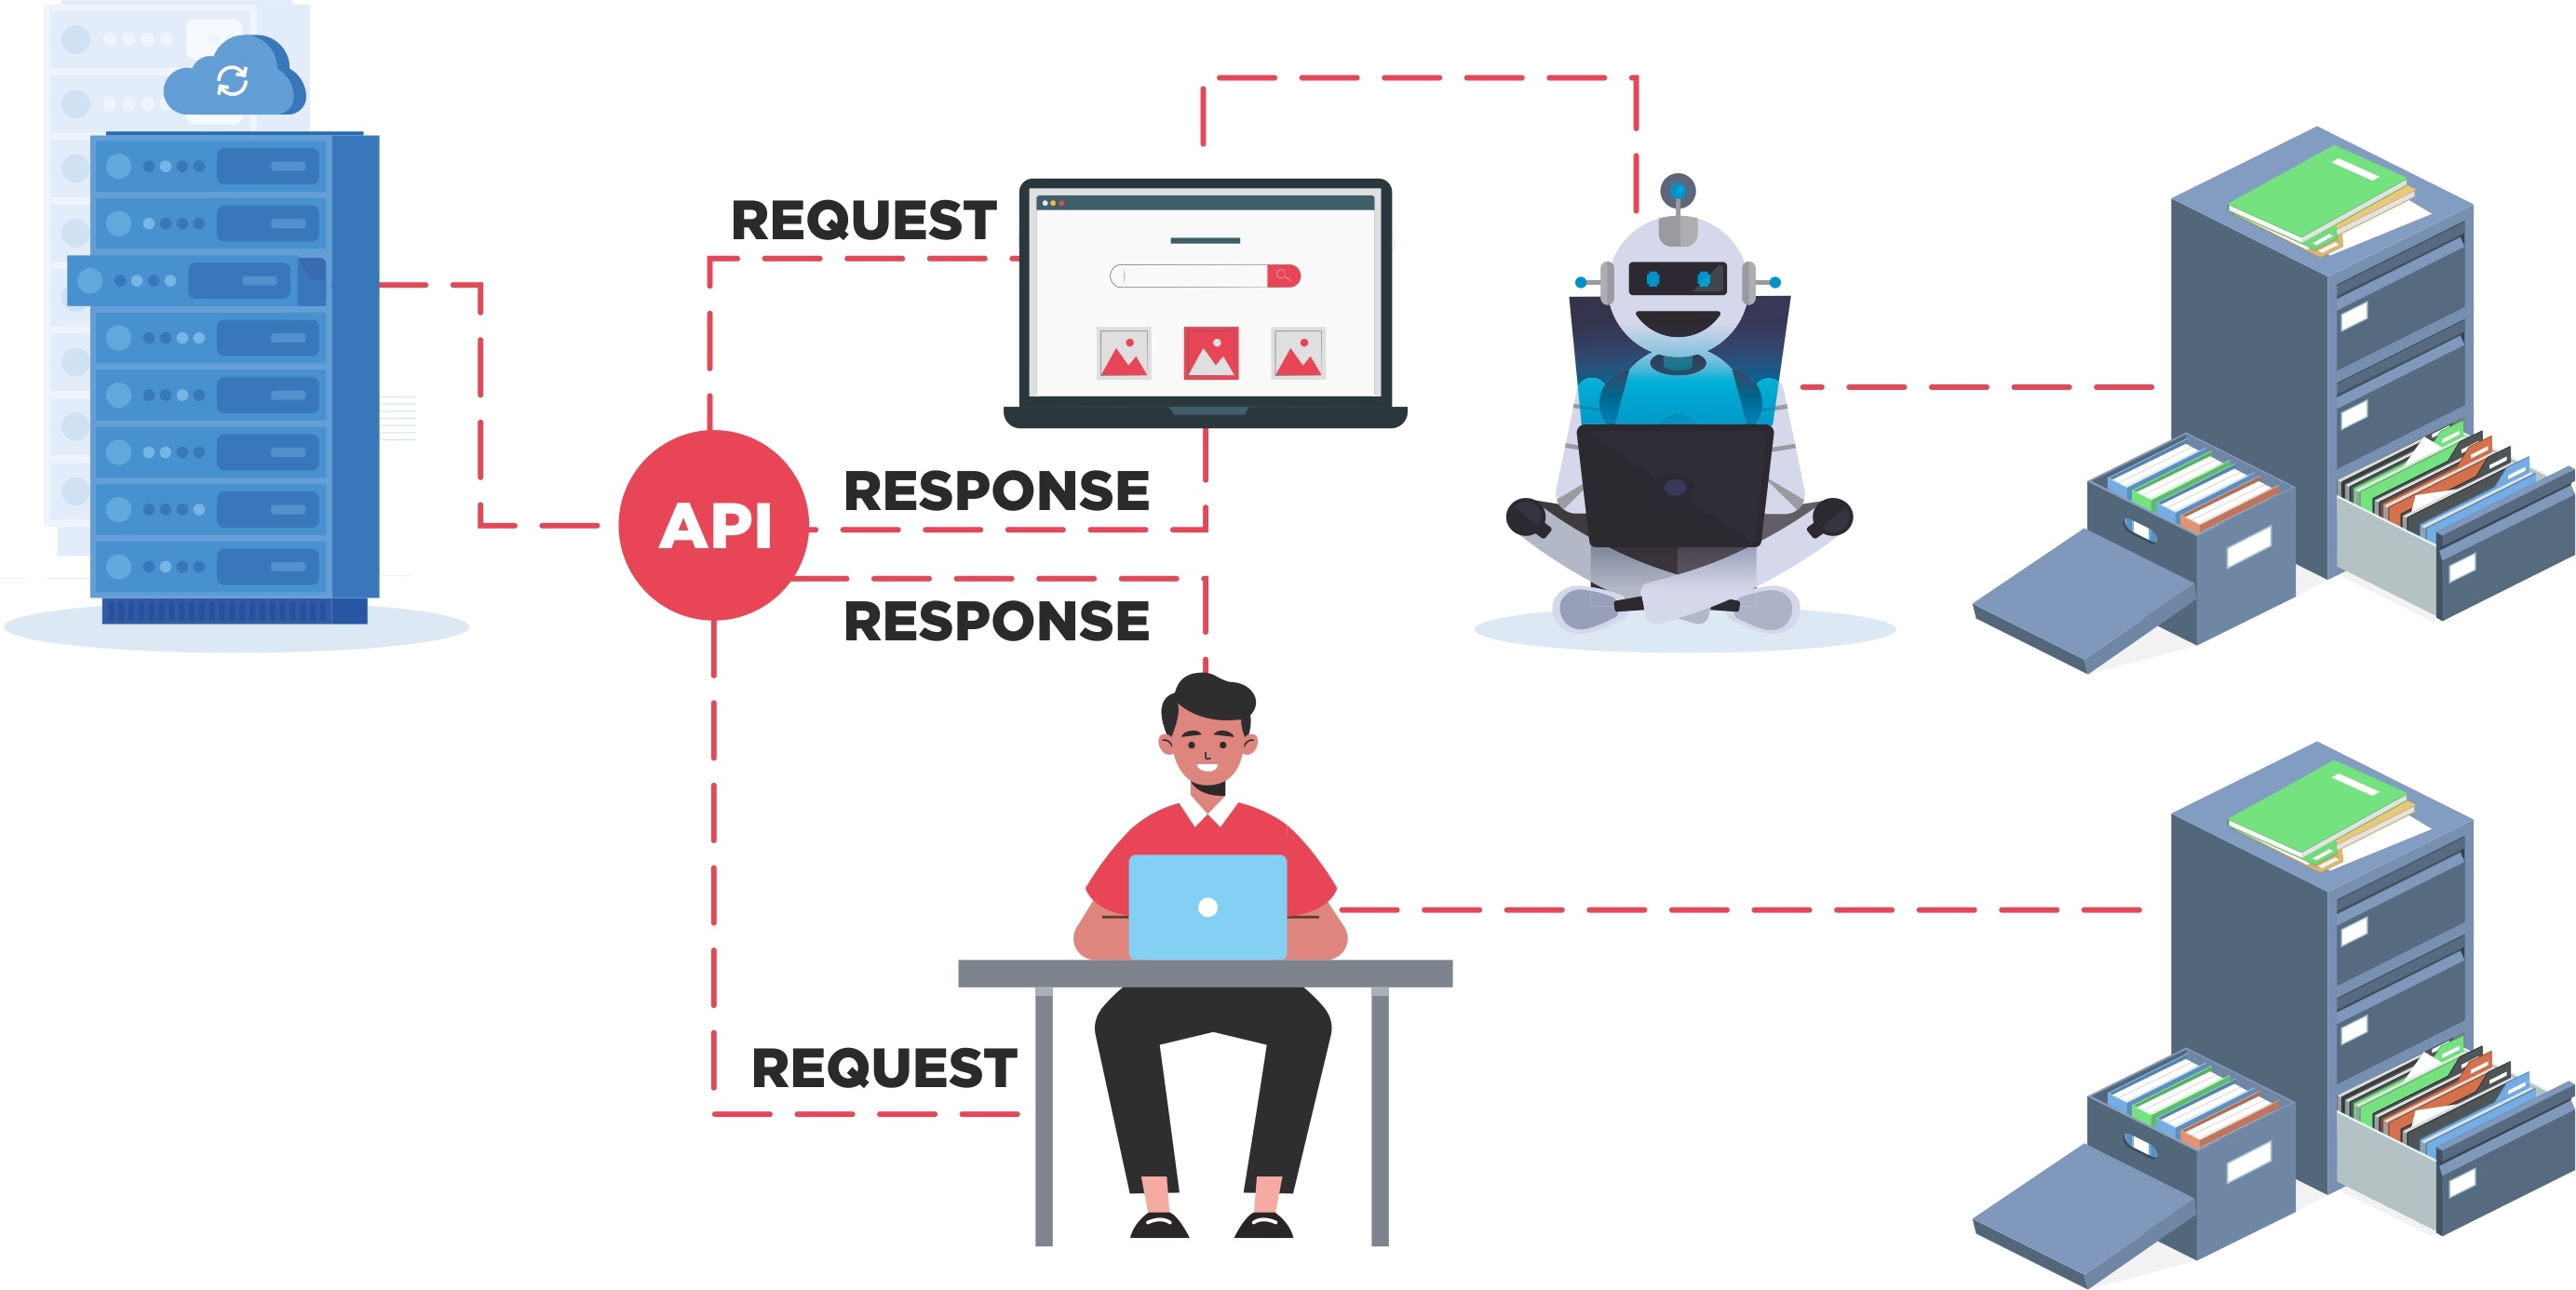
\includegraphics[scale = .4]{png/api.jpg}
        \end{figure}
    }
    \only<+>{
        \begin{figure}
            
\includegraphics[width = \textwidth]{png/twitter.png}
            \caption{from \textcolor{blue}{\href{https://developer.twitter.com/en/use-cases/analyze}{Developer X}}}
        \end{figure}
    }
    \only<+>{
        \begin{definition}
            \emph{Aplication Programming Interface} is a communication protocol between a client and a server intended to simplify the building of client-side software. In other words, it is a contract between the client and the server which defines the format of possible requests and the format of the response (i.e. format of the data).
        \end{definition}
    }
\end{frame}

\subsection[Data Formats]{Data Formats}

\begin{frame}
    \frametitle{Unstructured and Structured Data}
    \only<+>{
        \begin{figure}
            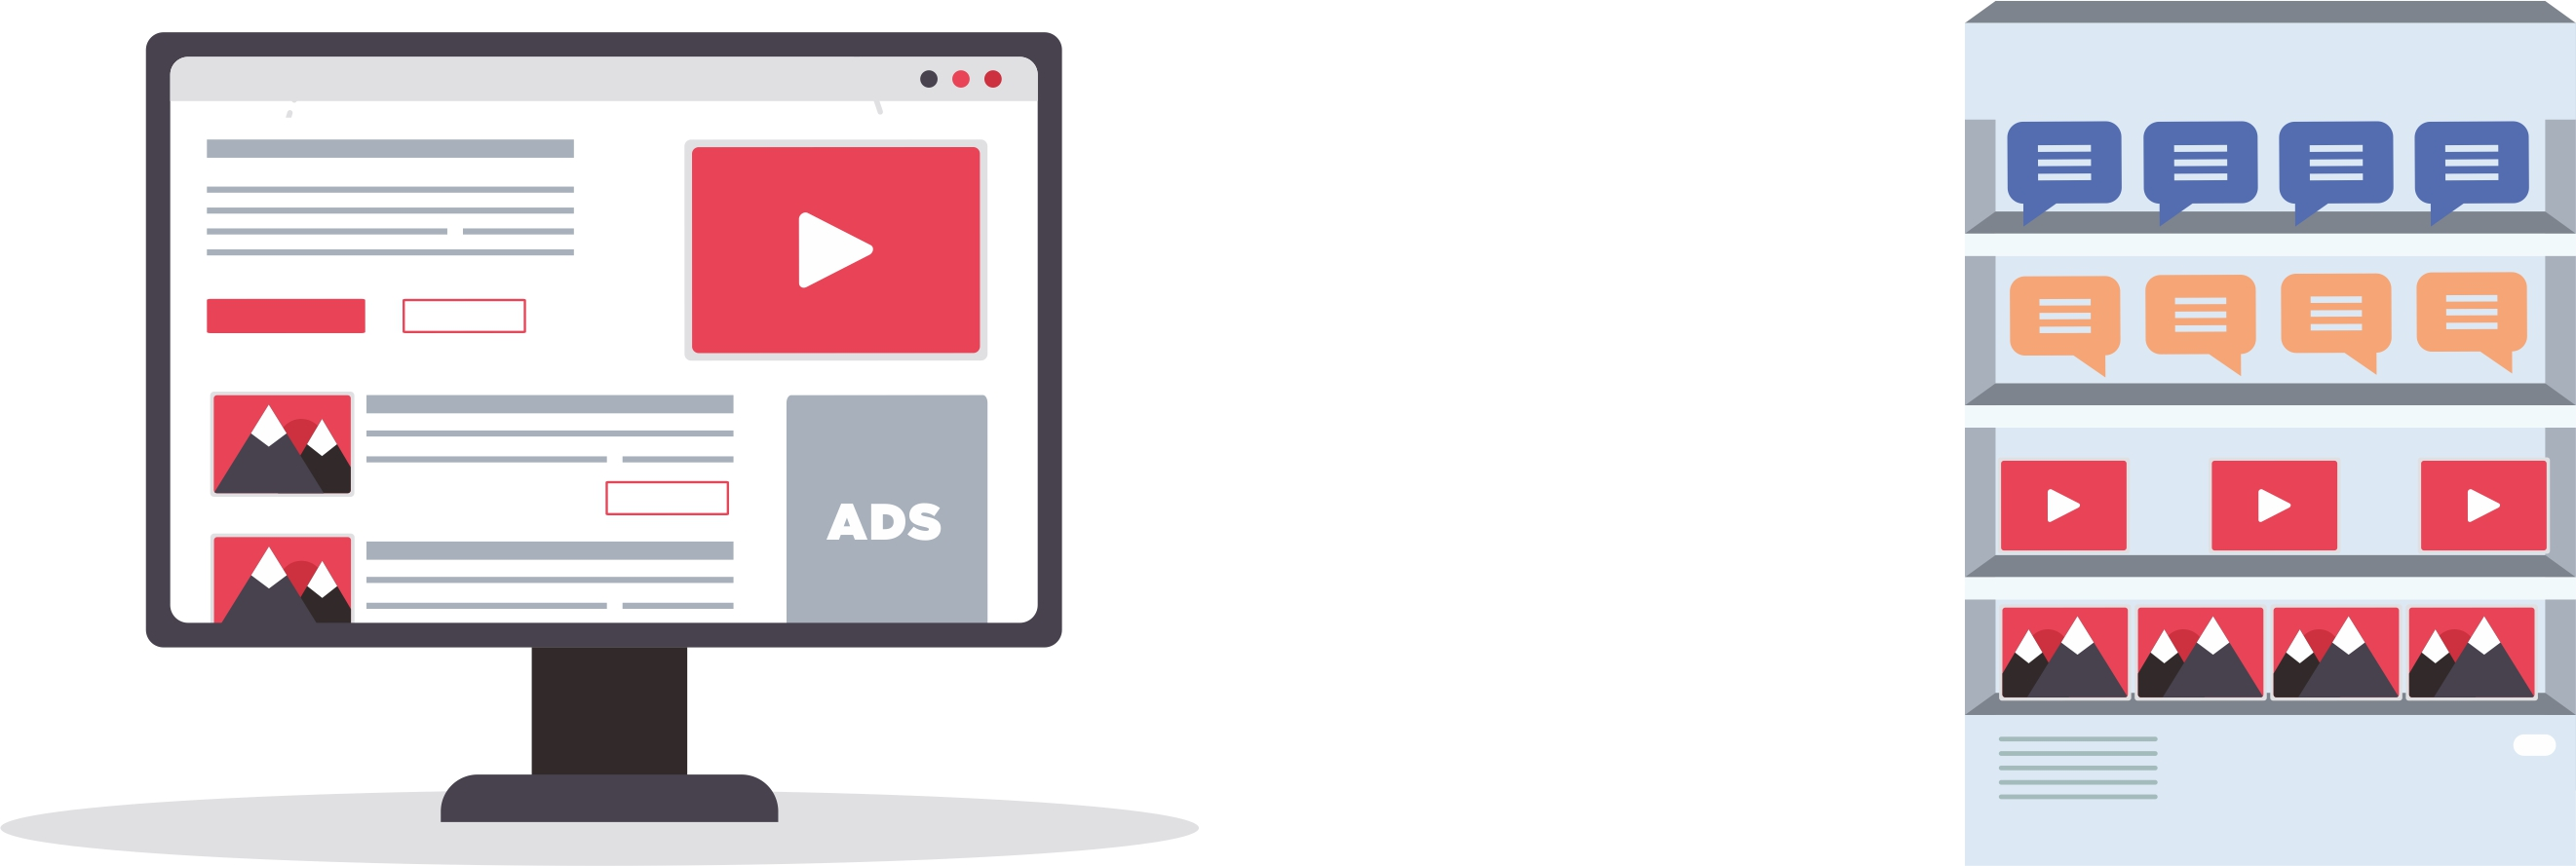
\includegraphics[scale = .4]{png/structured.jpg}
        \end{figure}
    }
    \only<+>{\begin{columns}[t]
        \begin{column}{.5\textwidth}
            Unstructured Data:
            \begin{itemize}
                \item can't be displayed in rows and columns
                \item images, audio, video, e-mails, spreadsheets, etc. (fun staff)
                \item requires more storage
                \item extremely hard to manage and analysis
            \end{itemize}
        \end{column}
        \begin{column}{.5\textwidth}
            Structured Data:
            \begin{itemize}
                \item can be displayed in rows and columns
                \item numbers, text, dates
                \item requires less storage
                \item easy to manage and analysis
            \end{itemize}
        \end{column}
        \end{columns}
    }
    \end{frame}
\begin{frame}
    \frametitle{Data Formats}
    \only<+>{
        Marianna is a 17 years old young lady. Although her main field of interest is physics (especially quantum physics and string theory), she also fancies sports. Her favorite physical activities are fishing and football.
        Marian, on the other hand, is a naughty 15 years old boy who only loves literature, especially Szymborska poems touch his heart.
    }
    \only<+>{
        \textcolor{red}{Marianna} is a \textcolor{blue}{17} years old young lady. Although her main field of interest is \underline{physics} (especially \textbf{quantum physics} and \textbf{string theory}), she also fancies \underline{sport}. Her favorite physical activities are \textbf{fishing} and \textbf{football}.
        \textcolor{red}{Marian}, on the other hand, is a naughty \textcolor{blue}{15} years old boy who only loves \underline{literature}, especially Szymborska \textbf{poems} touches his heart.
    }
    \only<+>{
        \resizebox{\textwidth}{!}{
            \begin{tabular}{l | c | c | c | c | c | c | c | c }
            Name & Sex & Age & Interest A & Interest A1 & Interest A2 & Interest B & Interest B1 & Interest B2\\
            \hline \hline
            Marianna & F & 17 & physics & quantum physics & string theory & sport & fishing & football\\
            Marian & M & 15 & literature & poems & n/a & n/a & n/a & n/a \\
            \end{tabular}}

    }
\end{frame}

\begin{frame}[fragile]{JSON - JavaScript Object Notation}
\begin{minted}[fontsize=\footnotesize]{js}
{
    "name": "Marianna",
    "age": 17,
    "interests": [
        {
            "name": "physics",
            "field": [
                "quantum physics",
                "string theory"
            ]
        },
        {
            "name": "sport",
            "field": [
                "fishing",
                "football"
            ]
        }
    ]
}
\end{minted}
\end{frame}

\begin{frame}[fragile]{JSON - JavaScript Object Notation}
\begin{minted}[fontsize=\footnotesize]{js}
{
    "name": "Marian",
    "age": 15,
    "interests": [
        {
            "name": "literature",
            "genre": [
                "poems"
            ]
        }
    ]
}
\end{minted}
\end{frame}

\begin{frame}
    \frametitle{JSON - JavaScript Object Notation}
    \begin{definition}
        \emph{JavaScript Object Notation} is a lightweight text data format that is relatively easy to read for both the human naked eye and computers. Although it derives from JavaScript it is a language-independent data format. JSON is built on two structures: a collection of key-item pairs and an ordered list of values. JSON filenames use .json extension.
    \end{definition}
\end{frame}


\begin{frame}[fragile]{JSON Lines}
\begin{minted}[fontsize=\footnotesize]{js}
{"name":"Marianna","age":17,"interests":[
    {"name":"physics","field":["quantumphysics","stringtheory"]},
    {"name":"sport","field":["fishing","football"]}
]}
{"name":"Marian","age":15,"interests":[
    {"name":"literature","genre":["poems"]}
]}
\end{minted}
\begin{definition}
    \emph{JSON Lines} (newline-delimited JSON) is a lightweight text data format that can be processed one record at a time. Each line consists of a JSON. JSON Lines filenames use .jl or .jsonl extensions.
\end{definition}
\end{frame}

\section[NLP]{Natural Language Processing}

\begin{frame}
    \frametitle{Natural Language Processing}
    \only<+>{
        \begin{figure}
            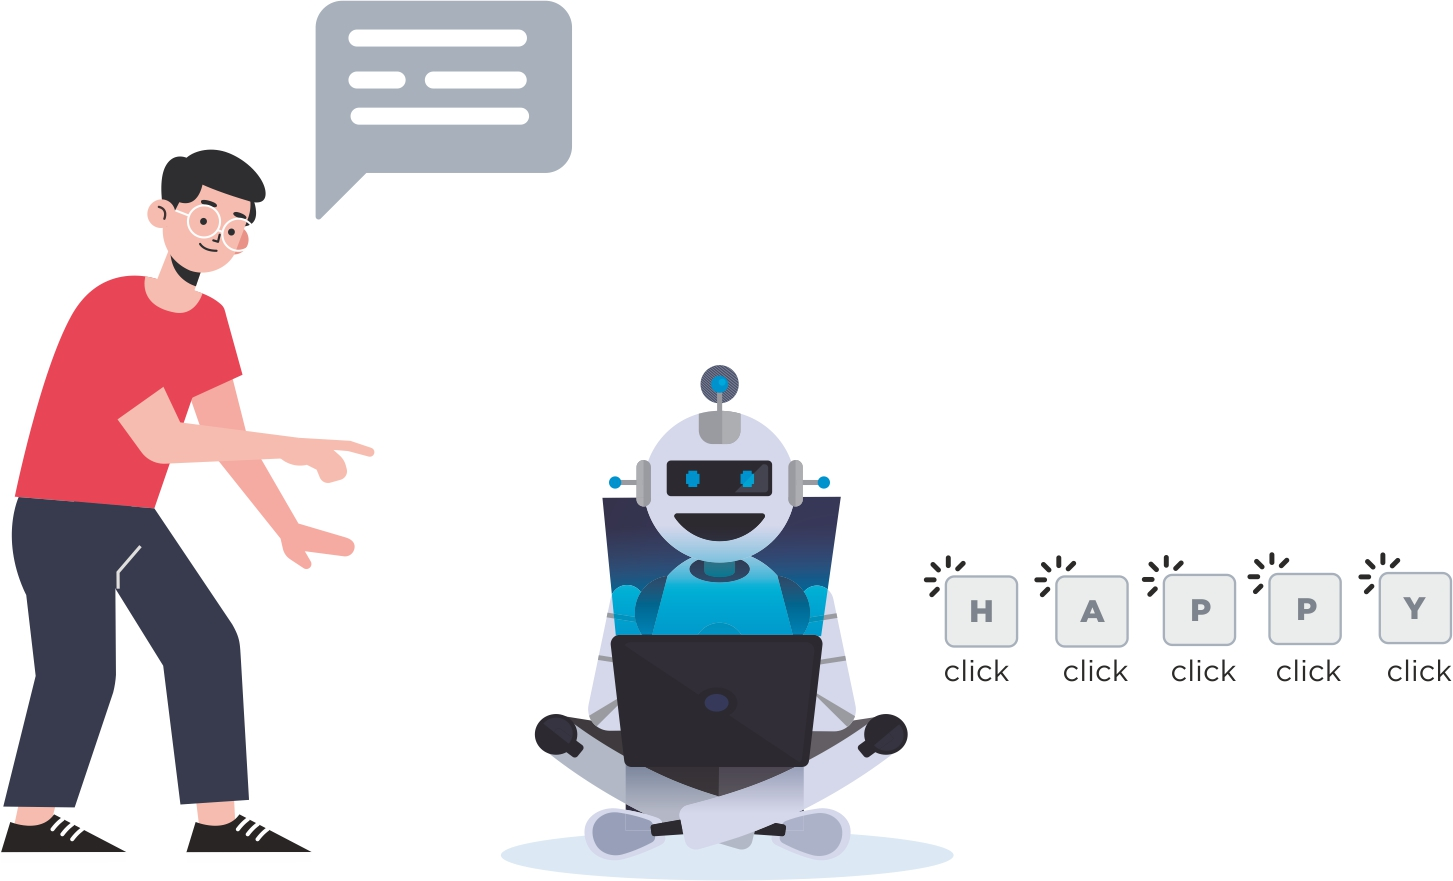
\includegraphics[scale = .7]{png/nlp.jpg}
        \end{figure}
    }
    \only<+>{
        \begin{definition}
            In a general sense \emph{Natural Language Processing} (NLP) is an analytical approach that uses a set of (usually) computer-based methods to extract meaning, topics, or sentiment from natural language data (written or spoken). In other words, it is a set of computer algorithms that tries to synthesize human language.  \end{definition}
    }
    \only<+>{
        \begin{itemize}
            \item tokenization
            \item stemming
            \item lemmatization
            \item sentiment analysis
            \item vector models
            \item topic modeling
            \item part of speech tagging
            \item entities analysis
    \end{itemize}
    }
\end{frame}

\begin{frame}
    \frametitle{For the next week}
    \begin{itemize}
       \item \textcolor{blue}{\href{https://www.theguardian.com/us-news/2015/dec/11/senator-ted-cruz-president-campaign-facebook-user-data}{Ted Cruz using firm that harvested data on millions of unwitting Facebook users}}
       \item Kosinski, M., Stillwell, D., \& Graepel, T. (2013). Private traits and attributes are predictable from digital records of human behavior. \textit{Proceedings of the National Academy of Sciences}, \textit{110(15)}, 5802–5805. \textcolor{blue}{\href{https://doi.org/10.1073/pnas.1218772110}{https://doi.org/10.1073/pnas.1218772110}}
    \end{itemize}
    
\end{frame}


\end{document}